\documentclass[journal]{IEEEtran}
\usepackage{cite}
\usepackage{amsmath,amssymb,amsfonts}
\usepackage{graphicx}
\usepackage{textcomp}
\usepackage{xcolor}
\usepackage{multirow}
\usepackage{booktabs}
\usepackage{url}

% NOTE: this file targets the OJSP track of ICASSP 2027 (8 pages of
% technical content + 1 references-only page, "short paper" category),
% which is reviewed and formatted as an IEEE Open Journal of Signal
% Processing (OJSP) submission rather than the standard 4+1-page ICASSP
% conference track. It therefore uses IEEEtran in journal mode (not the
% spconf/conference template used by the standard track), matching the
% OJSP author template obtained from the IEEE Author Center template
% selector. If the OJSP portal supplies an updated .cls/template at
% submission time, prefer that one and port only the content below
% \begin{document}.

\begin{document}

\title{A Longitudinal Comparison of Supervised and Reinforcement-Learning Decision Paradigms for sEMG Hand-Gesture Recognition}

\author{Luis-Gabriel~Mac\'ias-Santill\'an, Lorena~Isabel~Barona~L\'opez, Marco~E.~Benalc\'azar, and \'Angel~Leonardo~Valdivieso~Caraguay
\thanks{The authors are with the Artificial Intelligence and Computer Vision Research Lab, Departamento de Inform\'atica y Ciencias de la Computaci\'on (DICC), Escuela Polit\'ecnica Nacional, Quito, 170143, Ecuador.}}

\markboth{IEEE Open Journal of Signal Processing}{Mac\'ias-Santill\'an \MakeLowercase{\textit{et al.}}: A Longitudinal Comparison of Decision Paradigms for sEMG Hand-Gesture Recognition}

\maketitle

\begin{abstract}
Surface electromyography (sEMG) is non-stationary, yet most hand-gesture-recognition (HGR) systems are calibrated once and never re-evaluated across sessions. We report a six-month longitudinal study addressing two open questions: does a frozen deep representation shift over time independently of downstream accuracy, and does the choice between a supervised decision head and a reinforcement-learning-style one change how a system responds to that shift. We freeze a CNN-Transformer-encoder backbone (three capacities) after one calibration session and evaluate a supervised Softmax classifier and a LinUCB contextual bandit on six later sessions from 19 participants. Two independent two-sample tests detect statistically significant covariate shift in the frozen representation every month ($p<0.05$, Holm-Bonferroni-corrected), while accuracy falls only 4.6--5.9\% across all backbone-paradigm combinations, a band that does not widen as backbone capacity shrinks by two orders of magnitude. The representation drifts measurably; the resulting accuracy decline is governed by backbone capacity, not by decision paradigm; and a stable accuracy curve alone is not sufficient evidence that a longitudinal HGR system is unaffected by drift.
\end{abstract}

\begin{IEEEkeywords}
hand gesture recognition, surface electromyography, covariate shift, contextual bandits, Transformer encoder, longitudinal evaluation
\end{IEEEkeywords}

\section{Introduction}
\label{sec:intro}

\IEEEPARstart{S}{urface} electromyography (sEMG) is a widely used sensing modality for hand-gesture recognition (HGR), with applications in prosthetic control, rehabilitation, and human-machine interaction \cite{Jaramillo2020,Benalcazar2017}. sEMG signals are non-stationary: their statistics change across sessions due to electrode placement, fatigue, and skin impedance \cite{Montazerin2022,transradialSimon}. Despite this, most HGR studies still evaluate a model within a single session or under short-term cross-validation \cite{Jaramillo2020}, and reinforcement-learning-style decision mechanisms remain comparatively unexplored relative to supervised classifiers in this literature \cite{VasconezV2022,VASCONEZ2023}.

This leaves two questions largely untested with a formal procedure, rather than only assumed. First, if a deep feature extractor is frozen after calibration, does its output distribution actually shift over months, independently of whether downstream accuracy changes. This distinction matters in practice: a stable accuracy curve can mask a real shift if the decision head happens to compensate for it, so a system could be silently accumulating representational drift long before that drift becomes visible as an accuracy drop. Second, once a discriminative representation is learned, does the choice between a supervised decision head and a reinforcement-learning-style one change how the system responds to that shift. Contrasting two decision paradigms on an otherwise identical, frozen representation isolates this question in a way that contrasting two architectures cannot, since architecture changes would only speak to representation capacity, not to how a downstream decision rule handles a shifting input.

We answer both questions with a longitudinal design spanning six months. A CNN-Transformer-encoder backbone is trained once on session zero (Month~0) and frozen; its output is tested directly for covariate shift across six later monthly sessions with two independent two-sample tests, and separately scored with a supervised Softmax head and a LinUCB contextual bandit. We repeat the entire comparison at three backbone capacities, differing by two orders of magnitude in parameter count, to test whether any pattern we find is an artifact of one particular network size rather than a property of the representation-learning approach itself.

Our contributions are: (1) statistical evidence, from two independent two-sample tests jointly corrected for multiple comparisons, that a frozen deep sEMG representation exhibits covariate shift across six months even though this is largely invisible in the accuracy curve; and (2) a matched comparison of a supervised Softmax head against a LinUCB contextual bandit on the identical frozen representation, at three backbone capacities, showing that the resulting accuracy drop is governed by backbone capacity rather than by decision paradigm. Together, these results argue that a stable longitudinal accuracy curve should not, by itself, be read as evidence that a deployed HGR system is unaffected by representational drift, and that comparing decision paradigms in isolation from architecture capacity risks attributing a capacity effect to the wrong variable.

The remainder of this paper is organized as follows. Section~\ref{sec:method} describes the longitudinal protocol, signal preprocessing, backbone architecture, covariate-shift tests, and the two decision mechanisms in detail. Section~\ref{sec:results} reports the covariate-shift results and the accuracy comparison across paradigms and capacities. Section~\ref{sec:discussion} discusses the implications and limitations of these findings, and Section~\ref{sec:conclusion} concludes.

\section{Methodology}
\label{sec:method}

\subsection{Longitudinal Protocol}
Nineteen participants were recorded across seven sessions spanning six months (Month~0 through Month~6). Every model in this study is calibrated exactly once, on Month~0, and evaluated frozen (with no further parameter updates of any kind) on Month~1 through Month~6. This no-further-training rule is what makes it possible to attribute any accuracy change in a later month to the passage of time itself, rather than to the model having continued to learn from more data along the way.

Within Month~0, repetitions, not whole participants, are split 80/20 between training and validation, independently for each participant. This detail matters more than it might first appear: it guarantees that every one of the 19 participants contributes data to both the training set and the Month~0(val) evaluation set, and therefore also appears, unchanged, in every later month's evaluation set. As a direct consequence, the only variable that changes between the Month~0(val) baseline and the Month~1--6 evaluations is elapsed time; which participants are being evaluated never changes. Had the split instead been performed by participant (some participants entirely in training, others entirely in validation), any accuracy difference between Month~0(val) and later months could be explained just as easily by a train/validation population mismatch as by genuine temporal drift, and the two explanations could not be told apart from the accuracy numbers alone.

\subsection{Signal Preprocessing}
Eight-channel sEMG is amplitude-normalized, rectified, and low-pass filtered to obtain an envelope that tracks muscle activation without the raw signal's fast oscillation. The envelope is segmented into overlapping 300-sample frames with a 30-sample stride, and each frame is labeled against the annotated gesture interval by a dual-tolerance overlap rule: a frame is counted as belonging to the gesture if it covers at least 75\% of the frame's own duration with the annotated interval, or if it covers at least 50\% of the annotated interval's total duration, whichever of the two criteria is easier to satisfy for that particular interval. This dual criterion avoids systematically mislabeling frames near the boundary of short gesture intervals, where a fixed single threshold would otherwise discard a disproportionate share of valid frames. Each labeled frame is then converted to a $13\times24\times8$ spectrogram tensor (frequency bins by time bins by channel) via the short-time Fourier transform, which is the representation the backbone in Section~\ref{sec:backbone} consumes.

Frame-level class imbalance is substantial: roughly two-thirds of all frames belong to the \emph{noGesture} class, since a participant's hand spends more time at rest than mid-gesture during a recording session. We correct for this with balanced class weights, computed once from the Month~0 training data and then applied identically, without modification, to three otherwise-independent places: the backbone's cross-entropy loss during training, the Softmax head's loss, and the scale of the reward signal given to the LinUCB bandit (Section~\ref{sec:decision}). Using the same weights everywhere is a deliberate methodological choice: if the two decision mechanisms had instead used different class-weighting conventions, any accuracy difference between them could be explained by that difference alone, rather than by the decision paradigm itself.

\subsection{Transformer-Encoder Backbone}
\label{sec:backbone}
The feature extractor follows an Inception-style convolutional stage \cite{Isabel2023}, in which each block runs several parallel convolutional branches that extract features at different receptive-field sizes before their outputs are concatenated, folded into a single Transformer-encoder block \cite{Vaswani2017}. The full backbone is trained end-to-end with cross-entropy on Month~0 data only, and is then frozen at its final dropout layer. This freeze point yields a fixed-length representation $\mathbf{z}$ that is shared, unmodified, by both decision mechanisms described in Section~\ref{sec:decision}: after this point, neither the Softmax head nor LinUCB ever changes the backbone's weights, and neither receives a gradient signal that flows back into it. This backbone, at larger scale and trained on a substantially larger cohort, previously reached 95.25\% accuracy on a 612-participant sEMG dataset \cite{HGREncoder}; we cite that result to motivate this backbone's use here as an architecture with an established track record on this task, rather than as an untested design choice made for this study alone.

We train the same architecture at three capacities, differing only in width and depth, to test whether any effect reported in Section~\ref{sec:results} is an artifact of one particular network size rather than a property of the representation-learning approach itself: large (6 Inception blocks, embedding dimension $d_{model}{=}128$, 8 attention heads, 128-dimensional output), medium (4 blocks, $d_{model}{=}64$, 4 heads, 64-dimensional output), and small (2 blocks, $d_{model}{=}32$, 2 heads, 32-dimensional output). These three capacities span two orders of magnitude in parameter count. Every other training detail, including the loss function, the class-weight formula, the early-stopping rule, and the evaluation protocol, is held identical across the three capacities, so that capacity is the only variable that changes between them.

\subsection{Covariate-Shift Testing on the Frozen Representation}
\label{sec:covshift}
Before asking whether accuracy changes at all, we ask a more direct question: does the frozen representation $\mathbf{z}$ itself occupy a different region of feature space in later months than it did at calibration time. This distinction is not merely academic. A decision head that happens to compensate well for a real underlying shift can keep its accuracy curve essentially flat while the representation it is reading from has, in fact, moved substantially; testing $\mathbf{z}$ directly, independently of any classifier's downstream accuracy, is the only way to rule that scenario out and to know which of the two is actually happening.

We use two independent two-sample tests between Month~0 and each of the six later months, so that a shift found by only one of the two methods does not, by itself, drive our conclusions. Maximum Mean Discrepancy (MMD$^2$) is computed with a Gaussian RBF kernel, with the kernel bandwidth set by the standard median-heuristic rule \cite{Gretton2012MMD}. Separately, a domain classifier (logistic regression, 5-fold cross-validated) is trained to predict, from the 128-dimensional feature vector alone, whether a given sample comes from Month~0 or from month $m$; its cross-validated accuracy is then converted into the $\mathcal{H}$-divergence-based $\mathcal{A}$-distance, $d_{\mathcal{A}}=2(1-2\epsilon)$, where $\epsilon$ is the classifier's error rate \cite{BenDavid2010Domain}. This conversion has an intuitive reading at its two extremes: a domain classifier that performs at chance level ($\epsilon=0.5$) yields $d_{\mathcal{A}}=0$, meaning the two months' representations are statistically indistinguishable from each other, while a perfect classifier ($\epsilon=0$) yields $d_{\mathcal{A}}=2$, meaning the two months are fully separable. Both statistics are tested for significance with a 2000-iteration permutation test, and the twelve resulting $p$-values (six months times two tests) are jointly assessed with a Holm-Bonferroni correction for multiple comparisons, so that testing twelve hypotheses instead of one does not by itself inflate our chance of a false positive.

\subsection{Decision Mechanisms: Softmax and LinUCB}
\label{sec:decision}
A Softmax head, with $z$-score-normalized input, a weighted cross-entropy loss, and early stopping on Month~0 validation accuracy, instantiates the supervised paradigm: at every training step it is told the correct gesture label directly, and its loss is computed against that label. LinUCB \cite{Li2010LinUCB} instantiates a reinforcement-learning paradigm instead. It treats the frozen representation $\mathbf{z}_t$ at time $t$ as context and treats each of the six gesture classes as an arm to be chosen, selecting
\begin{equation}
\hat y=\arg\max_i \; \hat\theta_i^\top \mathbf{x}_t+\alpha\sqrt{\mathbf{x}_t^\top A_i^{-1}\mathbf{x}_t},
\label{eq:linucb}
\end{equation}
a predicted reward for arm $i$ plus an uncertainty bonus scaled by $\alpha$, and it updates its per-arm parameters $A_i$ and $\theta_i$ via a Sherman-Morrison rank-one update after observing only a scalar reward $r_t=\pm w_{c^*}$, where $w_{c^*}$ is the class weight of the true gesture $c^*$; the sign is positive if the chosen arm matched the true gesture and negative otherwise. LinUCB never observes the true label $c^*$ itself, only this scalar reward derived from it: this is the essential difference from Softmax, and the reason LinUCB is a genuine reinforcement-learning mechanism rather than a relabeled classifier wearing different notation. Under this update rule, LinUCB carries sublinear regret guarantees \cite{Chu2011Regret}.

Both mechanisms are warm-started exactly once, on Month~0, under the same kind of rule (shuffled-epoch training with early stopping on Month~0 validation accuracy), and are then frozen for the remainder of the study, exactly as the backbone itself is frozen. LinUCB additionally drops the uncertainty term $\alpha\sqrt{\mathbf{x}_t^\top A_i^{-1}\mathbf{x}_t}$ from Eq.~\eqref{eq:linucb} at evaluation time, since that term exists to drive exploration while a policy is still being learned, and has no defined purpose once learning has stopped. The two mechanisms' epoch budgets differ in absolute terms (Softmax: up to 200 epochs, patience 10; LinUCB: up to 20 epochs, patience 5), which reflects that a Sherman-Morrison update is computationally far cheaper per epoch than backpropagation through the Softmax head, not a difference in how generously each paradigm is allowed to converge. Despite this difference in raw epoch count, both mechanisms are stopped by the identical validation criterion (no further improvement in Month~0 validation accuracy) rather than by a fixed schedule chosen in advance. This equivalence in stopping rule, though not in epoch budget, is what lets us attribute any difference between the two paradigms in Month~1--6 (Section~\ref{sec:results}) to the decision paradigm itself, rather than to one paradigm having been cut off before it had a fair chance to converge.

\section{Results}
\label{sec:results}

\subsection{The Frozen Representation Shifts, With a Small Effect Size}
Fig.~\ref{fig:covshift} shows both covariate-shift statistics described in Section~\ref{sec:covshift}, computed for every one of the six later months. Both MMD$^2$ and the domain-classifier $\mathcal{A}$-distance reject the null hypothesis of no distributional difference at every single month ($p<0.05$), and this rejection survives a Holm-Bonferroni correction applied jointly across all twelve tests, including the single largest individual $p$-value in the set (Month~4, MMD test, $p=0.034$). At the same time, the domain classifier's cross-validated accuracy ranges only from 52.8\% to 59.4\% against a 50\% chance level, equivalently an $\mathcal{A}$-distance no larger than 0.38 out of a maximum possible value of 2. Taken together, this is the paper's central covariate-shift finding: the shift is statistically real by both independent tests, but its magnitude, as measured directly on the representation, is modest. Fig.~\ref{fig:covshift} also shows that neither statistic moves monotonically across the six months; MMD$^2$ reaches its highest value at Month~5 (0.00467) and its lowest at Month~4 (0.00048), a pattern we return to in Section~\ref{sec:discussion}.

\begin{figure}[t]
\centering
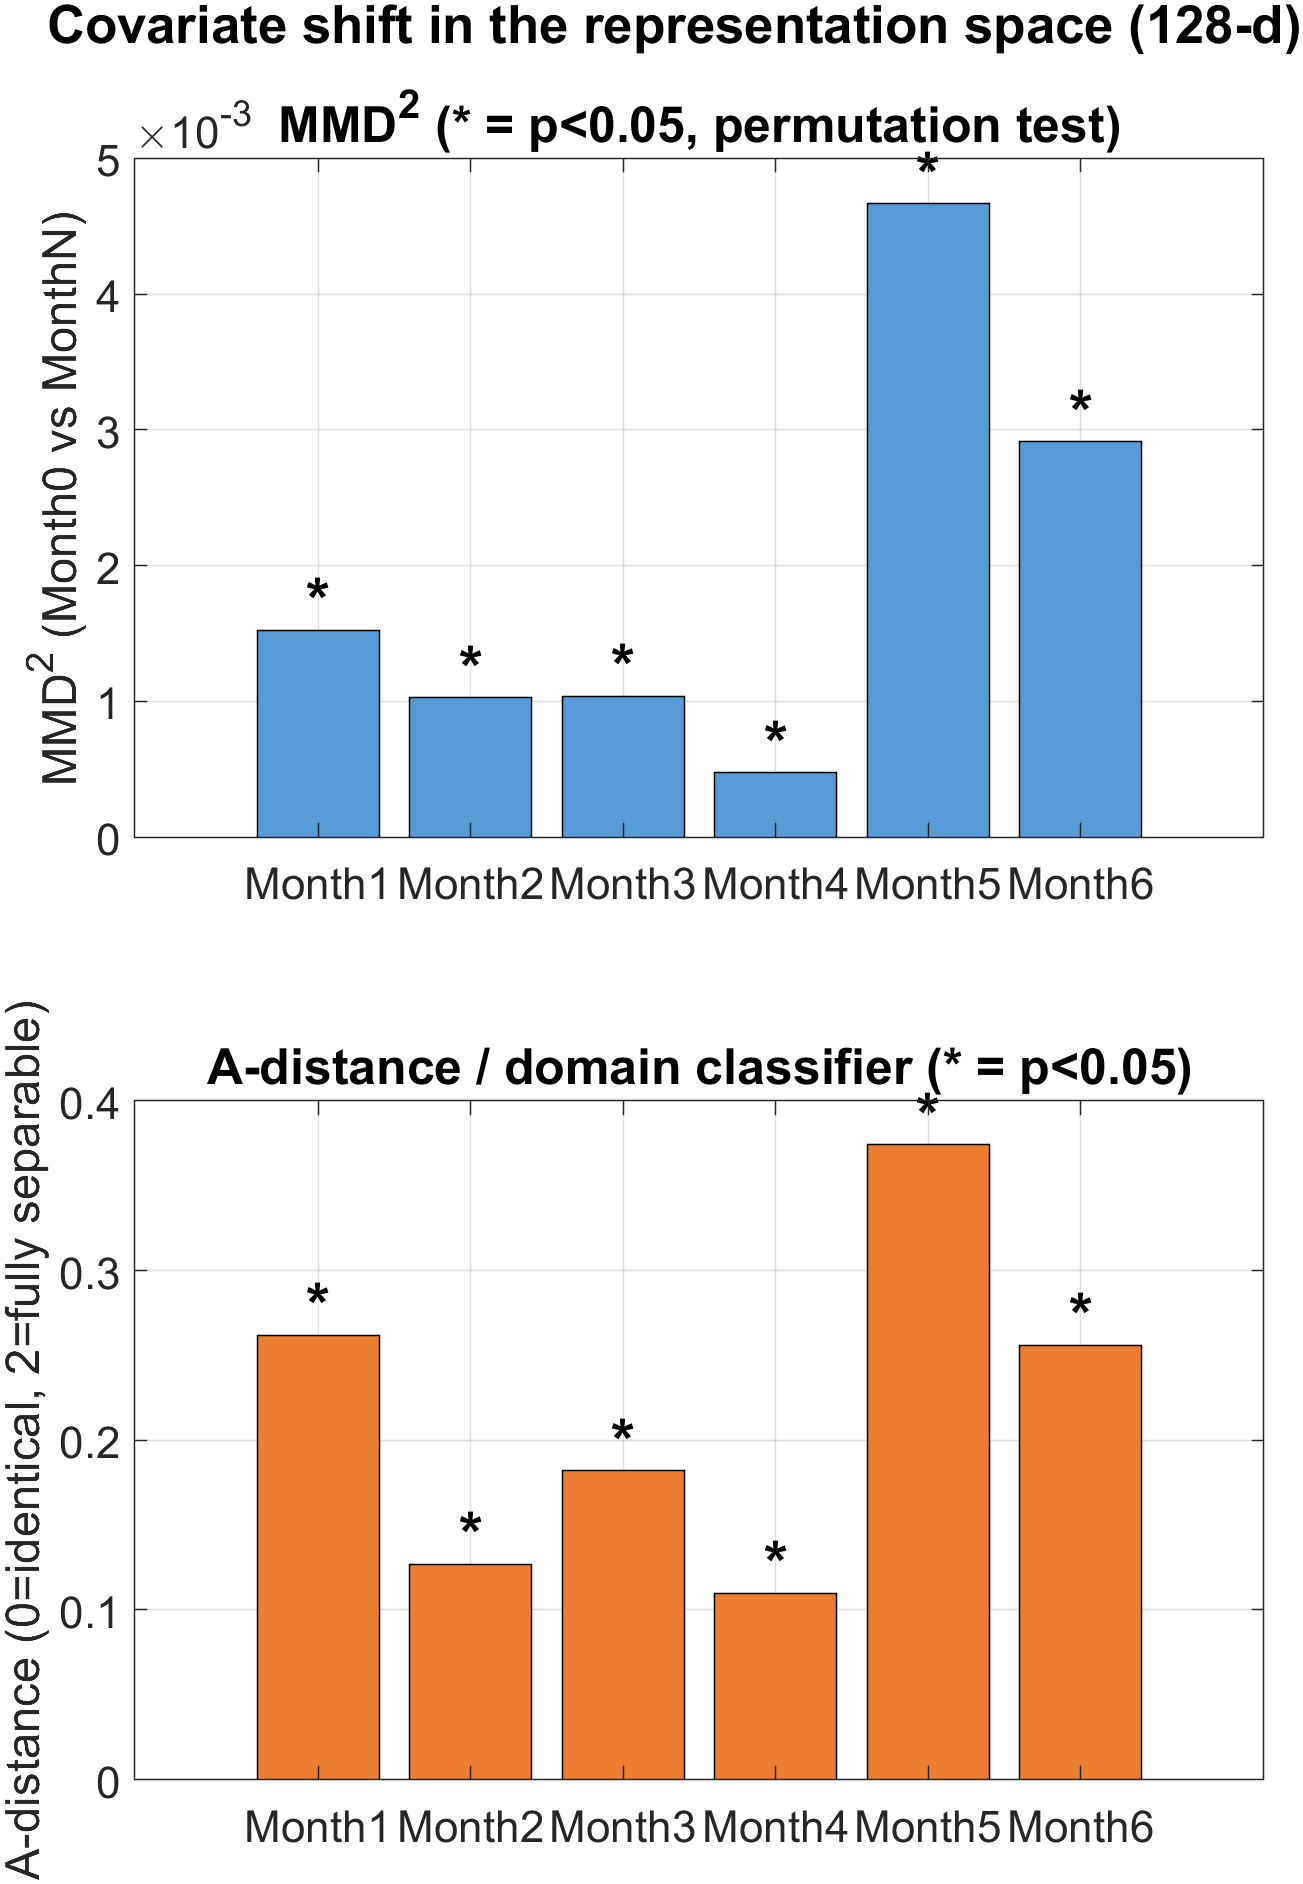
\includegraphics[width=\linewidth]{fig_covariate_shift_en.png}
\caption{MMD$^2$ (top) and domain-classifier $\mathcal{A}$-distance (bottom) between Month~0 and each later month. Asterisks mark $p<0.05$ after Holm-Bonferroni correction. Both statistics reject the null of no shift at every month, but neither moves monotonically, and the domain classifier stays close to chance level throughout.}
\label{fig:covshift}
\end{figure}

\subsection{Accuracy Drop is Governed by Backbone Capacity, Not by Decision Paradigm}
Having established that the representation itself shifts, we now ask how much this shift costs in accuracy, and whether that cost depends on the decision paradigm. Table~\ref{tab:results} reports Month~0(val)-to-Month~6 accuracy for both Softmax and LinUCB, at all three backbone capacities, together with the relative drop for each of the six backbone-paradigm combinations. Fig.~\ref{fig:sl_vs_rl} plots the full seven-session trajectory behind these two endpoint columns.

\begin{table}[t]
\caption{Accuracy at Month~0(val) vs.\ Month~6, and the relative drop, for both decision paradigms at three backbone capacities.}
\label{tab:results}
\centering
\begin{tabular}{@{}lcccccc@{}}
\toprule
\multirow{2}{*}{\textbf{Capacity}} & \multicolumn{3}{c}{\textbf{Softmax}} & \multicolumn{3}{c}{\textbf{LinUCB}} \\
\cmidrule(lr){2-4} \cmidrule(lr){5-7}
 & M0 & M6 & Drop & M0 & M6 & Drop \\
\midrule
Large  & 93.9 & 89.4 & 4.8\% & 93.3 & 87.8 & 5.9\% \\
Medium & 92.0 & 87.8 & 4.6\% & 91.3 & 87.0 & 4.8\% \\
Small  & 86.7 & 82.5 & 4.8\% & 84.6 & 80.7 & 4.6\% \\
\bottomrule
\end{tabular}
\end{table}

\begin{figure}[t]
\centering
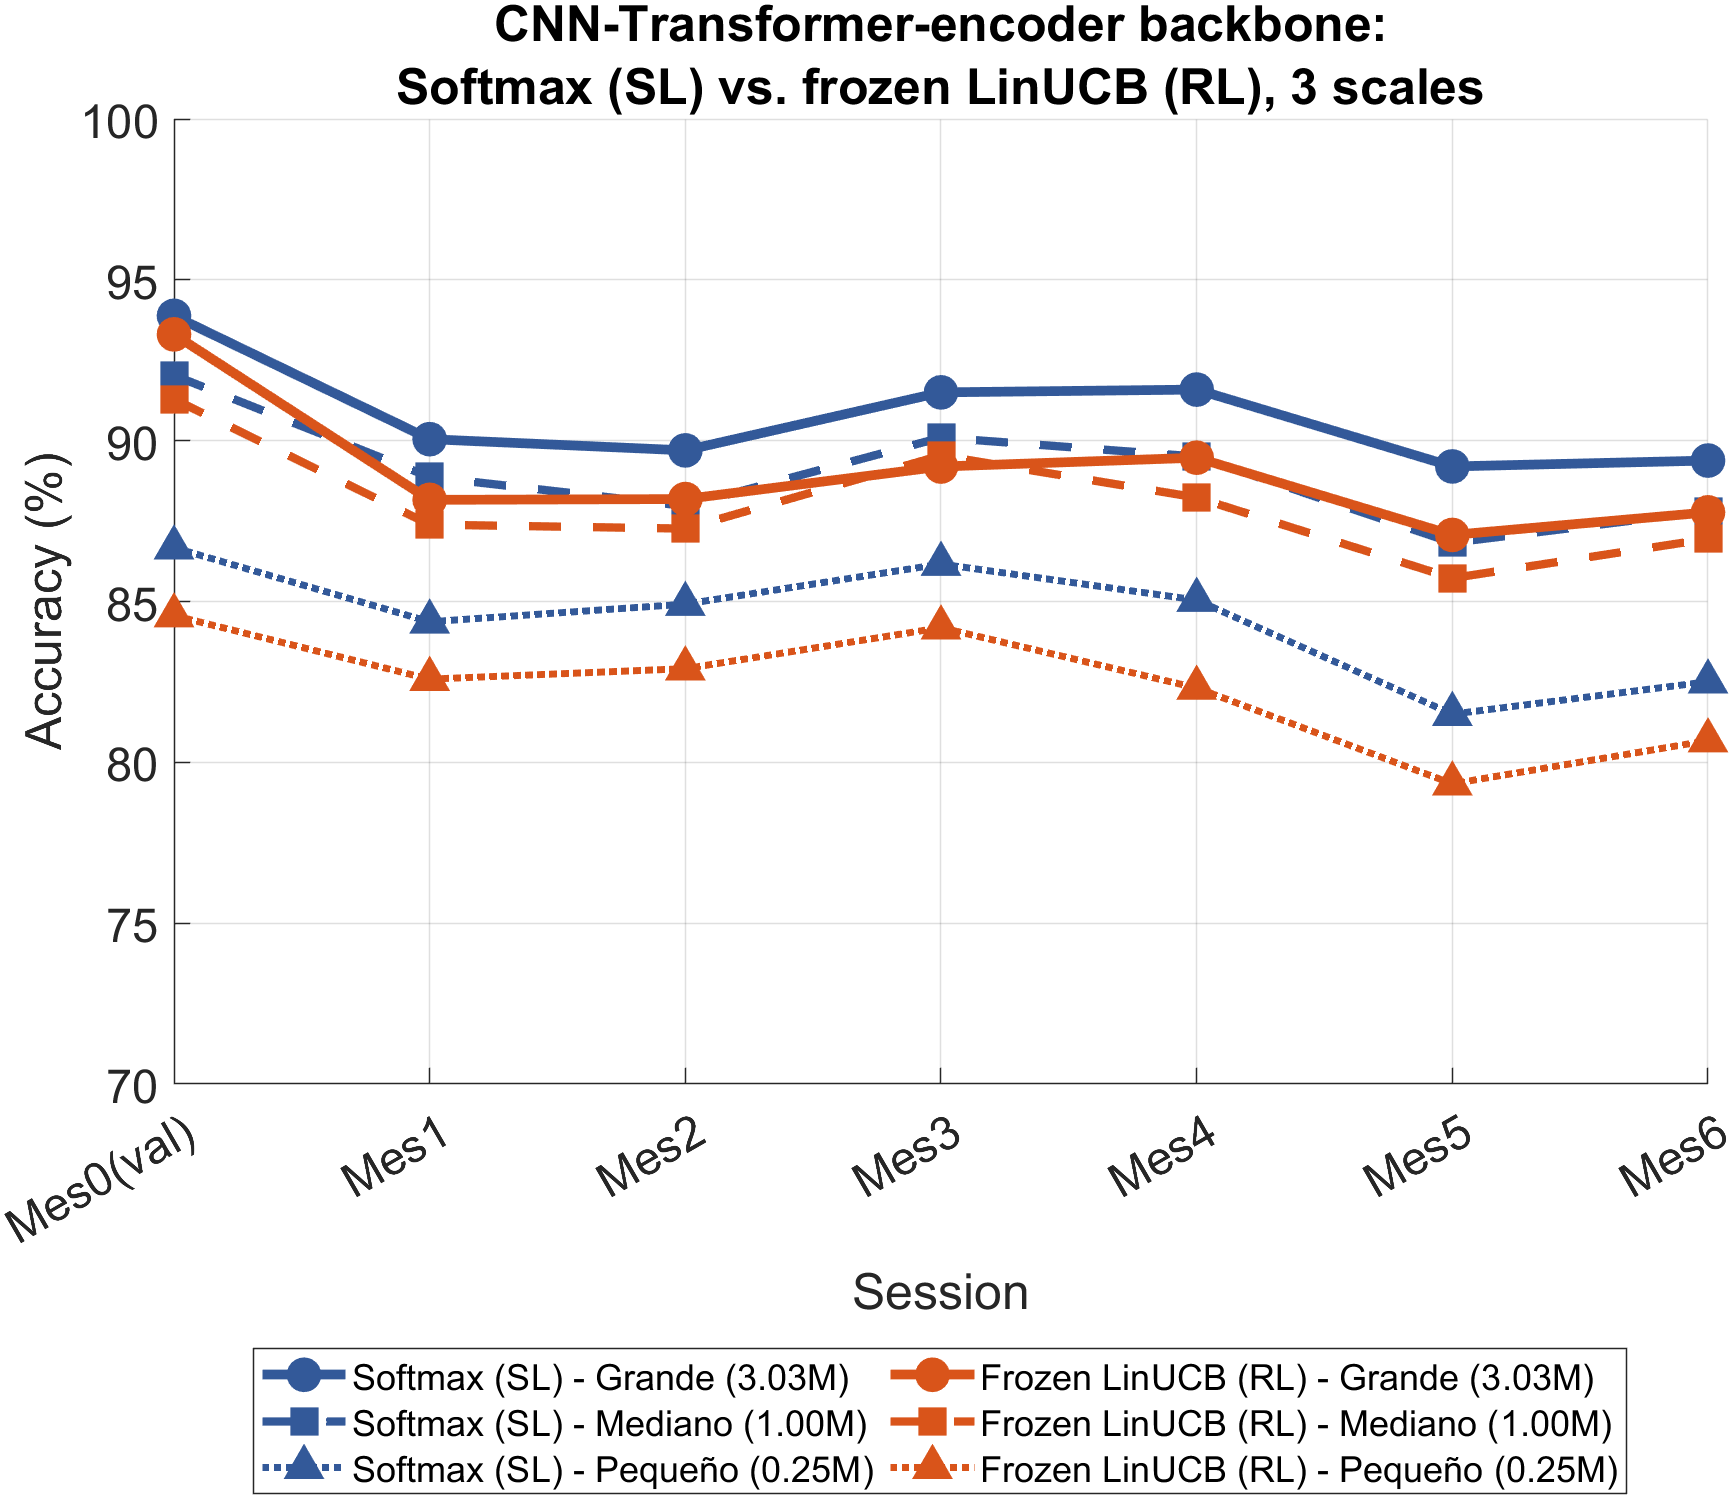
\includegraphics[width=\linewidth]{fig_sl_vs_rl_scales_en.png}
\caption{Accuracy across all seven sessions, Softmax vs.\ LinUCB, at three backbone capacities. The two paradigms track each other closely within each capacity; the separation between capacities is far larger than the separation between paradigms at any fixed capacity.}
\label{fig:sl_vs_rl}
\end{figure}

The drop is a narrow 4.6--5.9\% band regardless of capacity or decision paradigm, and Fig.~\ref{fig:sl_vs_rl} shows both paradigms tracking each other closely across all seven sessions and all three scales: at every capacity, the Softmax and LinUCB curves largely overlap, while the gap between the large, medium, and small curves is visually much larger than the gap between paradigms within any one capacity. Two observations follow directly from this pattern. First, because the 4.6--5.9\% band does not widen even as backbone capacity shrinks by two orders of magnitude (from a 128-dimensional representation down to 32-dimensional), capacity governs the absolute accuracy level, larger backbones reach higher accuracy at every session, but it does not govern how much either paradigm drifts away from its own Month~0 baseline. Second, because the drop is essentially the same magnitude whether the decision head is told the correct label directly, as Softmax is, or only a scalar reward, as LinUCB is, the decision paradigm itself does not appear to determine robustness to this shift; whatever mechanism drives the drop, it acts upstream of the paradigm-specific update rule, most plausibly in the representation itself, consistent with the direct covariate-shift evidence of Section~\ref{sec:results}A.

Every model's single largest step, in both Table~\ref{tab:results} and Fig.~\ref{fig:sl_vs_rl}, occurs between Month~0(val) and Month~1, rather than as part of a gradual month-over-month decline; accuracy is comparatively stable across Month~1 through Month~6 relative to that first step. Two design properties of the protocol, rather than a data artifact, explain most of this one-time step. First, Month~0(val) shares its recording session with Month~0(train): both come from the same sitting, the same electrode placement, and the same physiological state, while every one of Month~1 through Month~6 is, by construction, a new session with none of those held fixed. Second, every model's stopping point is selected by Month~0(val) accuracy (\texttt{ValidationPatience}, Section~\ref{sec:decision}), which mechanically favors whichever split is used for that selection; this is an unavoidable consequence of using validation accuracy for early stopping, not a flaw specific to one model. We could not fully separate this one-time session-identity effect from genuine month-over-month drift within the reported drop percentages using the data collected for this study, and we report this as an open methodological question for the field rather than apportion the two effects without direct supporting evidence.

\section{Discussion}
\label{sec:discussion}

Together, these results support a narrower and more precise claim than either of two broader claims a reader might otherwise reach for: that there is no drift at all, or that the decision paradigm is what determines robustness to drift. Neither broader claim survives contact with both pieces of evidence at once. A frozen sEMG representation shifts measurably, but modestly, across six months, and, critically, this shift is only visible when the representation itself is tested directly, as in Section~\ref{sec:results}A; it is largely invisible in the accuracy curve of Fig.~\ref{fig:sl_vs_rl}, which stays comparatively flat across the same six months. The resulting accuracy decline, in turn, is governed by backbone capacity, not by whether the decision head is a supervised classifier or a bandit. Taken together, this separates two claims that longitudinal HGR studies often conflate without stating either one explicitly: a stable accuracy curve is good evidence that a system tolerates a given amount of drift well in practice, but it is not, on its own, evidence that no drift occurred in the representation the system relies on. A system could look robust by this common measure while nonetheless resting on a representation that has already moved considerably from where it was calibrated.

This study has three limitations, each suggesting a concrete direction for future work. First, LinUCB is evaluated frozen and purely exploitative after its Month~0 warm-start; a permanently online, classifier-guided variant \cite{LinPaskettYang2025} was deliberately set aside here to keep both paradigms under matched, non-adaptive conditions for a fair comparison, but such a variant could behave differently under exactly the drift we document, since it would continue to receive reward signal throughout Month~1--6 rather than only during Month~0. Second, neither MMD$^2$ nor the accuracy drop moves monotonically across the six months, and we do not have a mechanistic explanation for this non-monotonicity; whether it reflects genuine non-monotonic physiological change, seasonal or behavioral confounds in the recording schedule, or simply noise at this sample size is a question this dataset cannot resolve on its own. Third, the backbone is trained once with cross-entropy and then frozen for the rest of the study; LinUCB never shapes the representation it operates on, so this study is not a test of end-to-end reinforcement learning, only of a reinforcement-learning-style decision rule applied on top of a representation trained by other means.

\section{Conclusion}
\label{sec:conclusion}

A frozen sEMG representation exhibits a small but statistically real covariate shift over six months, detected independently by two different two-sample tests and surviving correction for multiple comparisons. This shift corresponds to a modest 4.6--5.9\% accuracy decline that is consistent across three Transformer-encoder capacities spanning two orders of magnitude in parameter count, and consistent between a supervised Softmax head and a LinUCB bandit evaluated under matched conditions: decision paradigm does not change how much the system drifts, but backbone capacity does. Future work should test whether this pattern holds with the backbone trained end-to-end from reward alone, rather than frozen after supervised pretraining, whether it generalizes to other decision-head families beyond Softmax and LinUCB, and whether it holds at a larger participant cohort than the 19 studied here.

\section*{Data and Code Availability}
The longitudinal sEMG dataset used in this study is not publicly released: participant consent does not yet extend to unrestricted public redistribution (broadening it is in progress), and the dataset remains under active use by other ongoing studies in the same laboratory. It is available from the authors upon reasonable request. The complete analysis code is publicly available at \url{https://github.com/laboratorioAI/hgr-emg-longitudinal-study}.

\section*{Compliance with Ethical Standards}
All participants provided written informed consent prior to data collection, in accordance with the protocols of the Artificial Intelligence and Computer Vision Research Lab, Escuela Polit\'ecnica Nacional.

\section*{Acknowledgment}
The authors thank the Artificial Intelligence and Computer Vision Research Lab, Escuela Polit\'ecnica Nacional, for the data collection infrastructure used in this study.

% NOTE: using IEEEbib.bst (numbered IEEE citation style) since this
% repo does not carry the official IEEEtran.bst. Swap to IEEEtran.bst
% from the OJSP author kit if the submission portal requires the exact
% file; the citation format it produces is the same numbered style.
\bibliographystyle{IEEEbib}
\bibliography{bib}

\end{document}
